\chapter{Objects}

The following \emph{algebraic objects} (operators, monoids, and semirings) are presented in increasing generality.
The ``algebra generality rule'' of GraphBLAS states that a more general object can always be passed to
any method which requires a less general object. The restriction rules are explained in the respective sections of those objects.

Once algebraic objects (operators, monoids and semirings) are described, we introduce \emph{collections} (vectors, matrices and masks) that algebraic objects operate on. Finally, we introduce \emph{descriptors}, which are a simple way to do modify how algebraic objects operate on collections. More concretely, descriptors can be used (among other things) to perform multiplication with transpose of matrix without the user having to manually transpose the collection. A complete list of what descriptors are capable of can be found in the section.

\section{Operators}

A GraphBLAS \emph{binary operators} $F_b = \langle D_1, D_2, D_3, \odot \rangle$
is defined by three domains, $D_1$, $D_2$, $D_3$, and an operation
$\odot: D_1 \times D_2 \rightarrow D_3$.  For a given GraphBLAS operators
$F_b=\langle D_1, D_2, D_3,\odot \rangle$ we define $\bold{D}_1(F_b) = D_1$,
$\bold{D}_2(F_b) = D_2$, $\bold{D}_3(F_b) = D_3$, and $\bold{\bigodot}(F_b)
= \odot$.  Note that $\odot$ could be used in place of either $\oplus$ or $\otimes$.

A GraphBLAS \emph{unary operators} $F_u = \langle D_1, D_2, f\rangle$
is defined by two domains, $D_1$, $D_2$, and an operation
$f: D_1 \rightarrow D_2$.  For a given GraphBLAS operators
$F_u=\langle D_1, D_2, f \rangle$ we define $\bold{D}_1(F_u) = D_1$,
$\bold{D}_2(F_u) = D_2$, and $\bold{f}(F)
= f$.

\begin{table}
	\hrule
	\begin{center}
		\caption{Properties and recipes for building GraphBLAS algebraic objects: Unary Operator, Binary Operator, Monoid and Semiring (composed of operations Add and Times).\newline
			\hspace{\textwidth}Note 1: Output domain of Semiring Times must be same as domain of Semiring Add. This ensures 3 domains in total for Semiring rather than 4.}
		\label{Tab:Operator}
		
		\vspace{1\baselineskip}
		(a) Properties of algebraic objects.
		\vspace{1\baselineskip}
		
		\begin{tabular}{l|l|l|l}
			Object & Must Be Associative & Identity Must Exist & Number of Domains  \\
                        \hline
			Unary Operator & no & no & 2 \\
			Binary Operator & no & no & 3  \\
			Monoid & yes & yes & 1  \\
			Semiring Add & yes & yes  & 1  \\
			Semiring Times & no & no & 3  (Note 1) \\
		\end{tabular}
		
		\vspace{1\baselineskip}
		(b) Recipes for algebraic objects.
		\vspace{1\baselineskip}
		
		\begin{tabular}{l|l|l}
			Object          & Recipe                & Number of Domains  \\ 
                        \hline
			Unary Operator  & Function Pointer      & 2 \\				
			Binary Operator & Function Pointer      & 3  \\	
			Monoid          & Associative Binary Operator with Identity & 1  \\
			Semiring        & Associative Binary Operator with Identity $+$ &3 \\
                                        & Binary Operator &  \\
                        
		\end{tabular}
		
	\end{center}
	\hrule
\end{table}

\section{Monoids}

A GraphBLAS \emph{generalized monoid} (or \emph{monoid} for short) $M =
\langle D_1,\odot,0 \rangle$ is defined by a single domain $D_1$, an 
\emph{associative}\footnote{It is expected that implementations 
will utilize IEEE-754 floating point arithmetic which is not 
strictly associative.} 
operation $\odot: D_1 \times D_1 \rightarrow D_1$,
and an identity element $0 \in D_1$.  For a given GraphBLAS monoid $M=\langle
D_1,\odot,0 \rangle$ we define $\bold{D}_1(M) = D_1$, $\bold{\bigodot}(M) =
\odot$ and $\bold{0}(M) = 0$.  A GraphBLAS monoid is equivalent to 
the conventional \emph{monoid} algebraic structure.

Let $F = \langle D_1,D_1,D_1,\odot \rangle$ be a GraphBLAS binary operator
with element $0 \in D_1$.  Then $M = \langle F,0 \rangle = \langle
D_1,\odot,0 \rangle$ is a GraphBLAS monoid.

\section{Semirings}

A GraphBLAS \emph{semiring} (or \emph{semiring} for short)
$S=\langle D_1,D_2,D_3,\oplus,\otimes,0 \rangle$ is defined by
three domains $D_1$, $D_2$ and $D_3$, an \emph{associative}\footnote{It 
is expected that implementations will utilize IEEE-754 floating 
point arithmetic which is not strictly associative.} 
additive operation $\oplus : D_3 \times D_3 \rightarrow D_3$, 
a multiplicative operation $\otimes : D_1 \times D_2 \rightarrow
D_3$, and an element $0 \in D_3$.
For a given GraphBLAS semiring $S=\langle D_1,
D_2, D_3,\oplus,\otimes,0 \rangle$ we define $\bold{D}_1(S) = D_1$,
$\bold{D}_2(S) = D_2$, $\bold{D}_3(S) = D_3$, $\bold{\bigoplus}(S) =
\oplus$, $\bold{\bigotimes}(S) = \otimes$, and $\zero(S) = 0$. 

Let $F = \langle D_1,D_2,D_3,\otimes \rangle$ be a operator
and let $A = \langle D_3,\oplus,0 \rangle$ be a monoid,
then $S= \langle A,F \rangle = \langle D_1,D_2,D_3,\oplus,\otimes,0 \rangle$
is a semiring.

Note: There must be one GraphBLAS monoid in every semiring which 
serves as the semiring's additive operator and  
specifies the same domain for its inputs and output parameters. 

A UML diagram of the conceptual hierarchy of object classes in GraphBLAS
algebra (binary operators, monoids and semirings) is shown in 
Figure~\ref{Fig:AlgebraHierarchy}.

\begin{figure}[htb]
    \hrule
    \begin{center}
        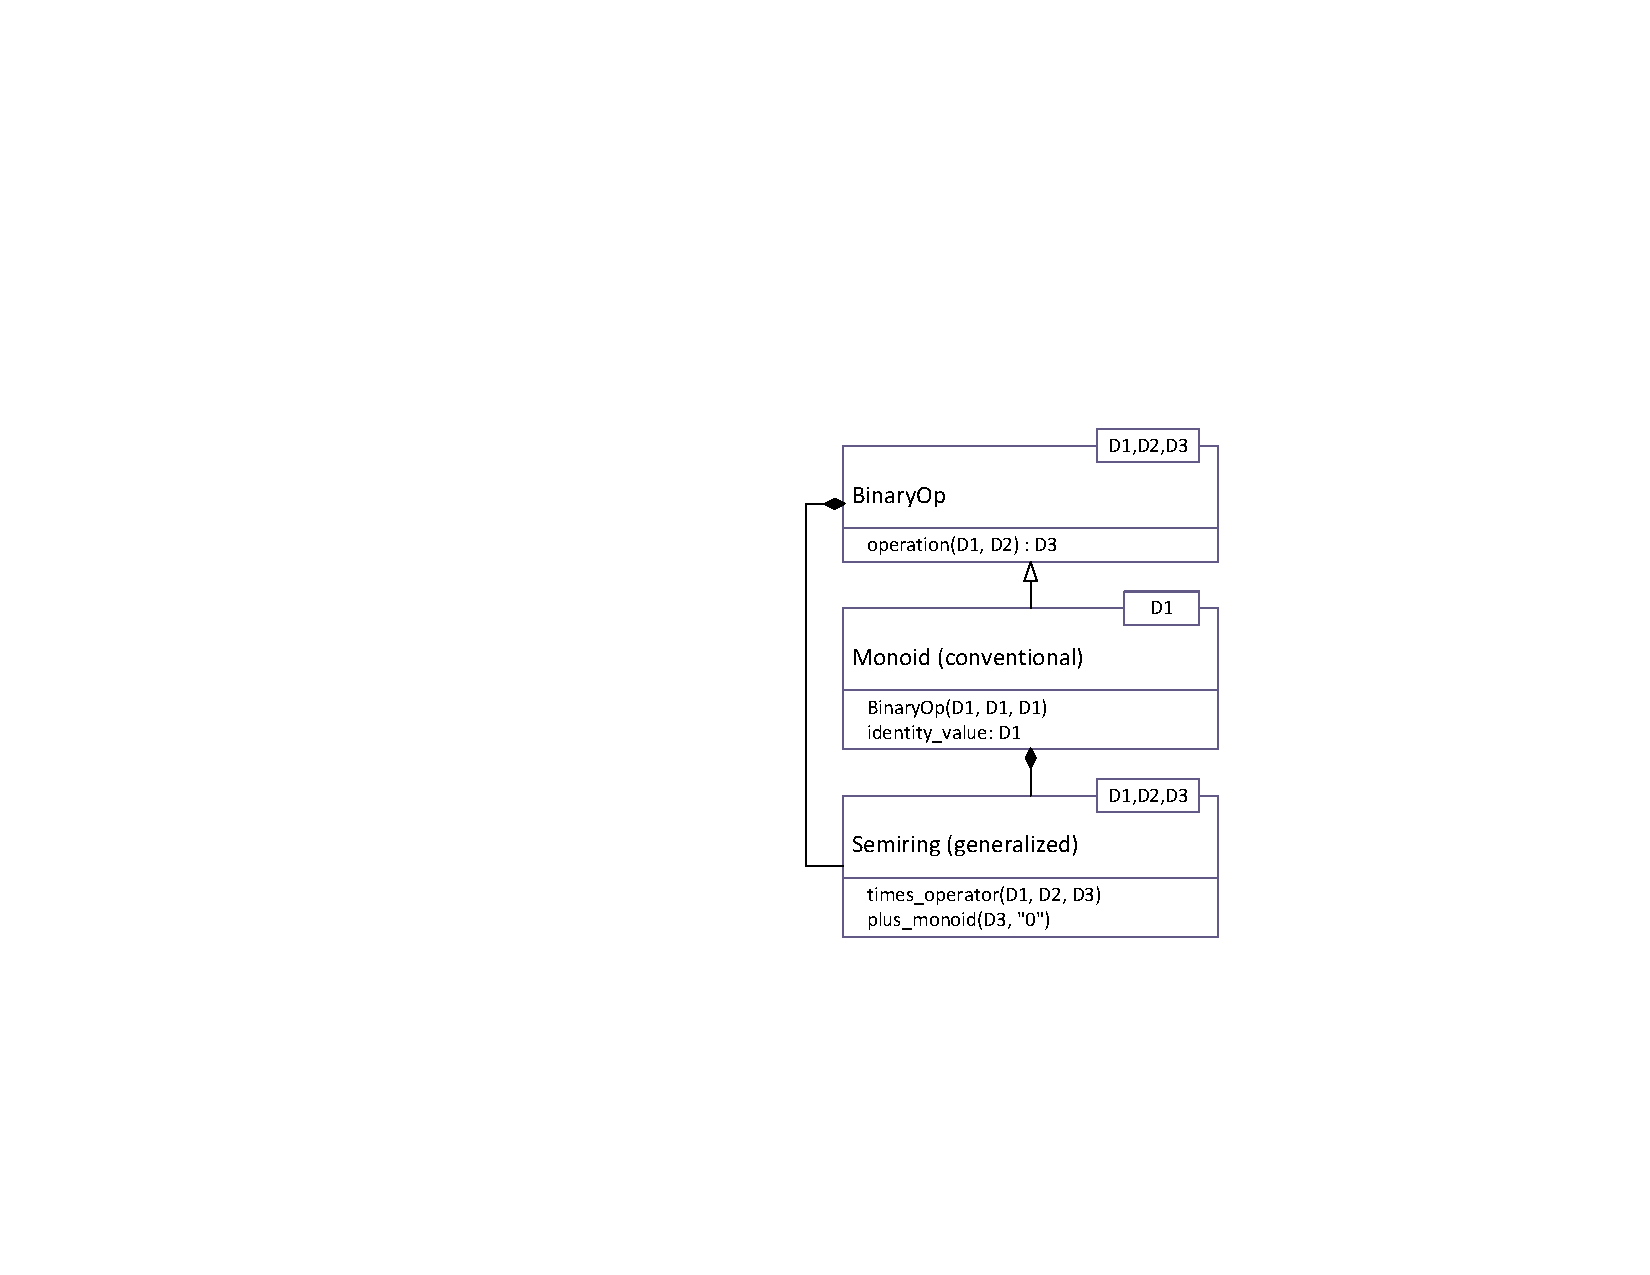
\includegraphics[width=1.0\linewidth,trim=3in 2in 0.5in 2in]{Algebra_Hierarchy_v2.pdf}
    \end{center}
    \caption{Hierarchy of algebraic object classes in GraphBLAS. GraphBLAS semirings consist of a conventional monoid with one domain for the 'add' function, and a binary operator with three domains for the 'multiply' function.}
    \label{Fig:AlgebraHierarchy}
    \hrule
\end{figure}

\begin{table}
    \hrule
    \begin{center}
        \caption{Proposed operator input for relevant GraphBLAS operations. 
        The semiring add and times are shown if applicable.}
        \label{Tab:OperatorInputType}
        \begin{tabular}{l|l}
        Operation           & Operator Input  \\ \hline
        {\sf mxm, mxv, vxm} & Semiring \\ \hline
        {\sf eWiseAdd}    & Monoid           \\
                            & Semiring          \\ \hline
        {\sf eWiseMult}     & Binary Operator   \\
                            & Monoid          \\
                            & Semiring         \\ \hline
  {\sf reduce} (to vector)  &  Binary Operator            \\ 
  					& Monoid           \\ \hline
  {\sf reduce} (to scalar)  & Monoid           \\ \hline
        {\sf apply}         & Unary Operator   \\ \hline
  {\sf buildMatrix} (dups)  & Binary Operator   \\
                            & Monoid           \\ \hline
{\sf accum} param, any op   & Binary Operator  \\
                            & Monoid            \\ 
        \end{tabular}
    \end{center}
    \hrule
\end{table}

\section{Vectors}
\label{Sec:Vectors}

A vector $\vector{v} = \langle D, N, \{ (i,v_i) \} \rangle$ is defined
by a domain $D$, a size $N>0$ and a set of tuples $(i,v_i)$ where
$0 \leq i < N$ and $v_i \in D$. A particular value of $i$ can only
appear at most once in $\vector{v}$. We define $\bold{n}(\vector{v}) =
N$ and $\bold{L}(\vector{v}) = \{ (i,v_i) \}$. The set $\bold{L}(\vector{v})$ is called
the \emph{content} of vector $\vector{v}$. We also define the set
$\vector{i(\vector{v})} = \{ i : (i,v_i) \in \bold{L}(\vector{v}) \}$,
and $\bold{D}(\vector{v}) = D$.

\section{Matrices}
\label{Sec:Matrices}

A matrix $\matrix{A} = \langle D, M, N, \{ (i,j,A_{ij}) \} \rangle$ is
defined by a domain $D$, its number of rows $M>0$, its number of columns
$N>0$ and a set of tuples $(i,j,A_{ij})$ where $0 \leq i < M$, $0 \leq
j < N$, and $A_{ij} \in D$. A particular pair of values $i,j$ can only
appear at most once in $\matrix{A}$. We define $\bold{n}(\matrix{A})
= N$,  $\bold{m}(\matrix{A}) = M$ and $\bold{L}(\matrix{A}) = \{
(i,j,A_{ij}) \}$.  
The set $\bold{L}(\matrix{A})$ is called the \emph{content} of matrix $\matrix{A}$.
We also define the sets $\vector{i(\matrix{A})} = \{
i : \exists (i,j,A_{ij}) \in \matrix{A} \}$ and $\vector{j(\matrix{A})}
= \{ j : \exists (i,j,A_{ij}) \in \matrix{A} \}$.  (These are the sets
of nonempty rows and columns of $\matrix{A}$, respectively.)  Finally,
$\bold{D}(\matrix{A}) = D$.

If $\matrix{A}$ is a matrix and $0 \leq j < N$, then $\matrix{A}(:,j)
= \langle D, M, \{(i,A_{ij}) : (i,j,A_{ij}) \in \bold{L}(\matrix{A})
\} \rangle$ is a vector called the $j$-th \emph{column}
of $\matrix{A}$. Correspondingly, if $\matrix{A}$ is a matrix and
$0 \leq i < M$, then $\matrix{A}(i,:) = \langle D, N, \{(j,A_{ij}) :
(i,j,A_{ij}) \in \bold{L}(\matrix{A}) \} \rangle$ is a vector called
the $i$-th \emph{row} of $\matrix{A}$.

\section{Masks}
\label{Sec:Masks}

A mask can be either a one- or a two-dimensional construct.
One- and two-dimensional masks, described more formally below, are
similar to vectors and matrices, respectively, except that they have
structure (indices) but no values. Masks are used to perform fine-grain control and optimization of GraphBLAS operations.

A one-dimensional mask $\vector{m} = \langle N, \{ i \} \rangle$
is defined by its number of elements $N>0$ and a set $\bold{L}(\vector{m})$ of indices $\{ i \}$ 
where $0 \leq i < N$.  A particular value of $i$ can only
appear at most once in $\vector{m}$. We define $\bold{n}(\vector{m}) = N$. 
We also define the set
$\vector{i(\vector{m})} = \{ i : i \in \bold{L}(\vector{m}) \}$.

A two-dimensional mask $\matrix{M} = \langle M, N, \{ (i,j) \} \rangle$,
is defined by its number of rows $M>0$, its number of columns
$N>0$ and a set $\bold{L}(\matrix{M})$ of tuples $(i,j)$ where $0 \leq i < M$, $0 \leq
j < N$.   A particular pair of values $i,j$ can only
appear at most once in $\matrix{M}$.  We define $\bold{n}(\matrix{M})
= N$, and $\bold{m}(\matrix{M}) = M$.  
We also define the sets $\vector{i(\matrix{M})} = \{
i : \exists (i,j) \in \bold{L}(\matrix{M}) \}$ and $\vector{j(\matrix{M})}
= \{ j : \exists (i,j) \in \bold{L}(\matrix{M}) \}$.  These are the sets
of nonempty rows and columns of $\matrix{M}$, respectively.

One common operation on masks is the \emph{structural complement}.  For a one-dimensional mask $\vector{m}$ this
is denoted as $\neg\vector{m}$. For a two-dimensional
masks this is denoted as $\neg\matrix{M}$.
The structure of the complement of an one-dimensional mask $\vector{m}$ is
defined as $\bold{L}(\neg\vector{m}) = \{i : 0 \leq i < N, i \notin \bold{L}(\vector{m}) \}$.
It is the set of all possible indices that do not appear in $\vector{m}$.
The structure of the complement of a two-dimensional mask $\matrix{M}$ is
defined as $\bold{L}(\neg\matrix{M}) = \{(i,j)$ : $0 \leq i < M$, $0 \leq
j < N$, $(i,j) \notin \bold{L}(\matrix{M}) \}$.  It is the set of all possible
indices that do not appear in $\matrix{M}$.

\section{Descriptors}

Descriptors are used as input parameters in various GraphBLAS methods to
provide more details of the operation to be performed by those methods.
In particular, descriptors specify how the other input parameters
should be processed before the main operation of a method is performed.
A Descriptor is a lightweight object with a collection of flags
for various modifiers for the other arguments.  Each type of argument
(vectors, matrices, masks, accum functions, etc.) have a different set of
valid flags.

For example, a descriptor may specify that a particular input matrix
needs to be transposed or that a mask needs to be structurally complemented 
(defined in Section~\ref{Sec:Masks})
before using it in the operation.  Some methods may also allow additional
processing of the result before generating the final output parameter.

For the purpose of constructing descriptors, the parameters of a method
are identified by specific names. The output parameter (typically
the first parameter in a GraphBLAS method) is {\sf OUTP}.  The mask is 
almost always next and is named {\sf MASK}. The input parameters (but
not the operations) are named {\sf ARG0}, {\sf ARG1}, {\sf ARG2} and so 
on from the first input parameter to the last. Finally, the descriptor
(typically the last parameter in a method) is not named, since GraphBLAS
does not support modifications of descriptors themselves.
